\documentclass[xcolor=table, 9pt]{beamer}
\mode<presentation>{}
\usepackage{beamerthemesplit} 

\setbeamertemplate{footline}[frame number]
\setbeamertemplate{headline}{}

\usepackage[english]{babel}
\usepackage[utf8x]{inputenc}
%\usepackage{xcolor}
\usepackage{makecell}
\usepackage[vlined,linesnumbered,titlenumbered,algoruled]{algorithm2e}
\usepackage{amsmath}


\title[PPT - Game Theory Path Planner]{A Game-theoretic Path Planner for Handling Uncertain Environment Forecasts}
\author{Evan Krell}
\institute{Texas A\&M University - Corpus Christi}
\date{November 2018}

\begin{document}

\begin{frame}
  \titlepage
\end{frame}

\begin{frame}{Outline}
  \tableofcontents
\end{frame}

\begin{section}{Introduction}
    \begin{frame}{Introduction}
        \begin{center}
            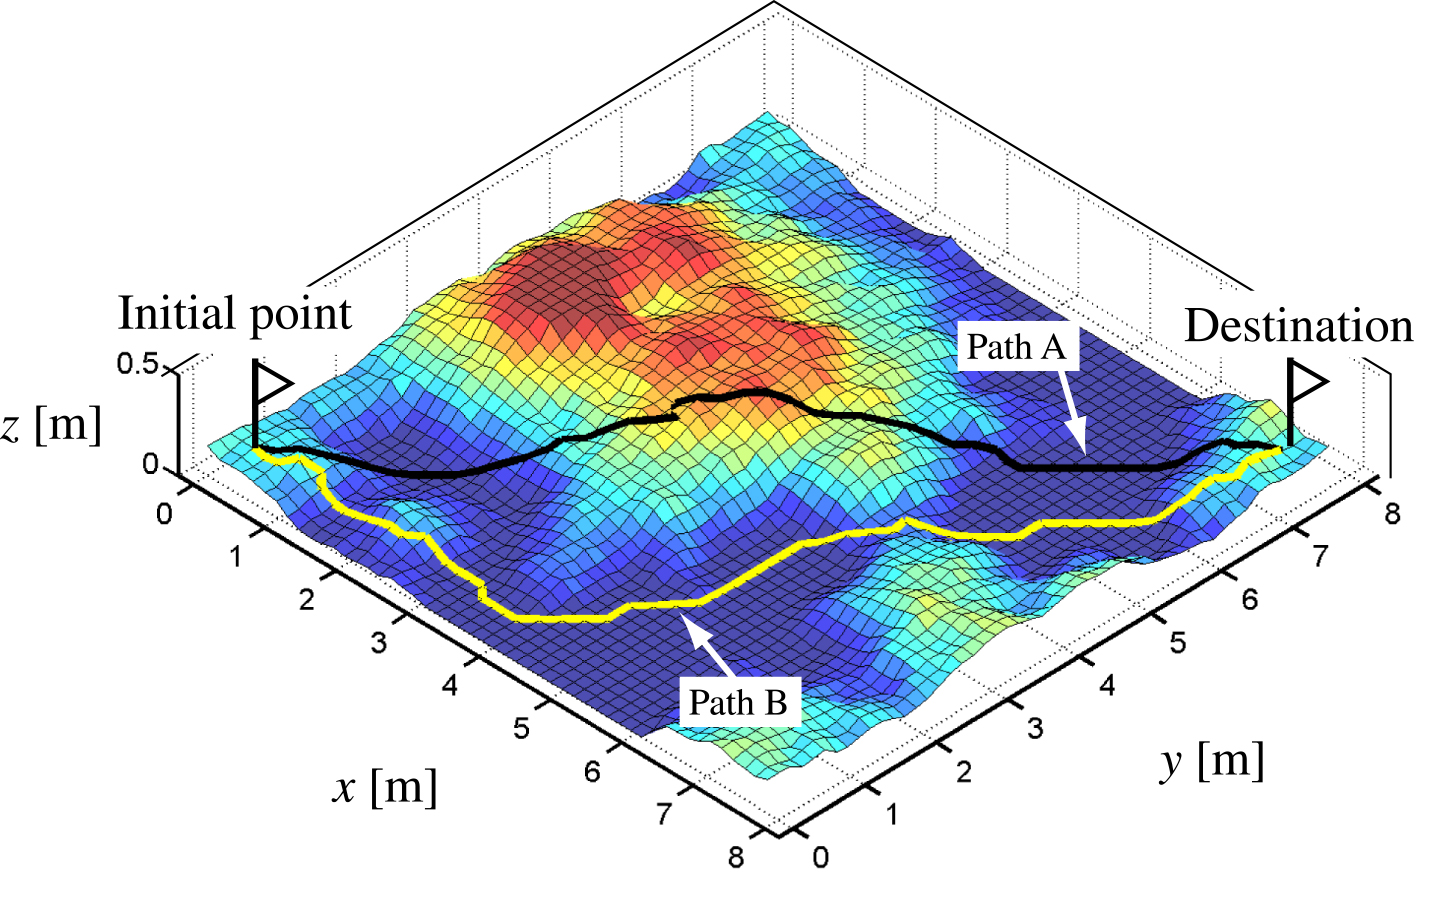
\includegraphics[width=\textwidth,trim={0cm 0cm 0cm 0cm},clip]{img/path.jpg} \\
            Image: \url{astro.mech.tohoku.ac.jp/~ishigami/research/path_plan.html}
        \end{center}        
    \end{frame}
    \begin{frame}{Introduction}
        \begin{block}{Dynamic Programming Path Planning}
            \begin{itemize}
                \item Solution at each cell, rather than single path
                \item Iterative \& approximate
                \item First iteration gives feasible, suboptimal plan; others improve it
            \end{itemize}
        \end{block}
        \begin{block}{Game Theory Path Planning}
            \begin{itemize}
                \item Handles uncertainty in environment predictions
                \item Each cell has zero-sum matrix game between traveler and environment
                \item Nash equilibrium for regret-free plan even in worst conditions
            \end{itemize}
        \end{block}
        \begin{block}{Previous Work}
            \begin{itemize}
                \item S. M. LaValle: \textit{Robot Motion Planning: A Game-Theoretic Foundation}
                \item Jasna, et al: \textit{Application of game theory in path planning of multiple robots}
            \end{itemize}    
        \end{block}
    \end{frame}
\end{section}

\begin{section}{Methods}
    \begin{frame}{Methods}
        \begin{block}{Dynamic Programming Path Planning}
            \begin{itemize}
                \item Applicable when subsolutions of final solution are themselves solutions for reduced problem
                \item Memoization: Store solved subsolutions for later access
                \item Bottom-up: Solve smallest subsolution, then expand toward final solution 
            \end{itemize}
            \begin{table}[]
\begin{tabular}{|l|l|l|l|l|}
\hline
$\searrow$ & $\searrow$  & $\downarrow$   & $\swarrow$     & $\swarrow$   \\
\hline
$\searrow$ & $\searrow$  & $\downarrow$   & $\swarrow$     & $\swarrow$   \\
\hline
$\rightarrow$ & $\searrow$  & $\downarrow$   & $\swarrow$     & $\swarrow$   \\
\hline
\textbf{X}           &   \textbf{X}  & $\swarrow$  & $\swarrow$    & $\swarrow$  \\
\hline
\textbf{O}  & $\leftarrow$  & $\leftarrow$ & $\leftarrow$ & $\leftarrow$ \\
\hline
\end{tabular}
\caption{Solution as vector field of action to take at cell}
            \end{table}
            
        \end{block}
    \end{frame}
    \begin{frame}{Methods}
        \begin{block}{Game Theory Path Planning}
            \begin{itemize}
                \item Theory: chapter on dynamic games 
                \item Exactly like Closed Loop, but over predictions
                \item Discrete intervals of environment's choices in error range
                \item \textbf{Flat matrix:} Combinations of multiple forces are single column
            \end{itemize}
            \begin{table}[]
            \small
\begin{tabular}{|l|l|l|l|l|l|l|l|l|l|l|}
\hline            
Halt         & INF & INF & INF & INF & INF & INF & INF & INF & INF & INF \\
\hline
$\uparrow$    & 8346 & 8346 & 8346 & 8347 & 8347 & 8348 & 8348 & 8348 & 8349 & 8349 \\
\hline
$\downarrow$   & 8291 & 8291 & 8290 & 8290 & 8289 & 8289 & 8289 & 8288 & 8288 & 8287 \\
\hline
$\leftarrow$  & 8349 & 8349 & 8348 & 8348 & 8347 & 8347 & 8347 & 8346 & 8346 & 8345 \\
\hline
$\rightarrow$ & 8332 & 8332 & 8332 & 8333 & 8333 & 8334 & 8334 & 8335 & 8335 & 8336 \\
\hline

\end{tabular}
\caption{Game between traveler (4-way moves) and environment with 10 error choices}
            \end{table}            
        \end{block}
    \end{frame}
    \begin{frame}{Methods}
        \begin{block}{Nash Equilibrium Solver - Raymond Hettinger}
            \begin{itemize}
                \item Approximate (\textit{fast}) iterative solver 
                \item \url{code.activestate.com/recipes/496825-game-theory-payoff-matrix-solver/}
                \item Successive plays $\rightarrow$ countermoves $\rightarrow$ proportions as mixed strategy
                \item \textbf{Deterministic:} Convert mixed solution to pure strategy
            \end{itemize}
            \begin{algorithm}[H]
            \caption[NashSolver]{\textbf{NashSolver:} Hettinger's 0-sum 2-player solver} 
            \label{alg:nashSolver}
            \SetAlgoVlined
            \KwIn{game $G$, iterations $i$}
            \KwOut{mixed policies for $P_i \& P_2$}
            Init $P_1$ policy  $\leftarrow$ 0-vector\;
            Init $P_2$ policy  $\leftarrow$ 0-vector\;
            Set $P_1$, $P_2$ action $\leftarrow$ 1\;
            \For{each iteration}{
                $P_1$ action  $\leftarrow$ counter-action to $P_2$ action\;
                $P_2$ action  $\leftarrow$ counter-action to $P_1$ action\;
                Increment values at each players mixed policies for current actions\;
            }
            Divide both mixed policies by $i$\;
            \Return {$P_1$ policy, $P_2$ policy}
            \end{algorithm}
        \end{block}
    \end{frame} 
    \begin{frame}{Methods}
        \begin{block}{Program Features}
            \begin{itemize}
                \item \textit{N} environment forces
                \item Each has weight, error
                \item Errors either scalar or matrix where each cell has specific error
                \item Generate waypoints from any start point
                \item Input region, force vectors as geotiff
                \item Saves solution for generating multiple paths
                \item Accepts forces as either (magnitude, direction) or (u, v)-components
            \end{itemize}
        \end{block}
    \end{frame}
\end{section}
\begin{section}{Mathematical Formulation}
    \begin{frame}{Mathematical Formulation}
        \begin{block}{Region Formulation}
            \begin{itemize}
            \item M := number of rows in region
            \item N := number of columns in region
            \item J := number of force vectors affecting region
            \item Occupancy Grid $O := M \times N$ matrix where
            \begin{itemize}
                \item Value of 1 indicates occupied
                \item Value of 0 indicates free
            \end{itemize}
            \item Force Grids (u components) $F^u := \{F^u_1 .. F^u_J\}$ where each is an $M \times N$ matrices of forces applied at cell.
            \item Force Grids (v components) $F^v := \{F^v_1 .. F^v_J\}$ where each is an $M \times N$ matrices of forces applied at cell.
            \item Error Grids $E := \{E_1 .. E_J \}$ are the $M \times N$ errors or each force
            \item $E_i \in E$ is error range of $F^u_i$ and $F^v_i$
            \item $x_{goal} :=$ coordinates of goal in region
            % \item Weights $W = \{W_i .. W_j\}$ are scalar weights of each force 
            \end{itemize}
        \end{block}
    \end{frame}
    \begin{frame}{Mathematical Formulation}
        \begin{block}{Game Formulation}
            \begin{itemize}
            \item Players $P := \{P^1 :=$ \textit{traveler}, $P^2 :=$ \textit{environment}\}
            \item Stages $K := \{1 ... M \times N\}$, where each cell is a stage
            \item Action space for $P^1, U := \{U^1 .. U^B_K\}$, $B$ is number of actions. 
            \begin{itemize}
                \item 4-way: \{halt, up, down, left, right\}
                \item 8-way: \{halt, up, down, left, right, up-left, up-right, down-left, down-right\}
            \end{itemize}
            \item Action space for $P^2, \Theta := \{\Theta^1_1 .. \Theta^A_K\}$, $A$ is the number of discrete actions.
            \item Control action $\theta^\alpha_k := $ tuple of selected f and v components for each force.
            \item State $x_k := (row, col)$ used to index appropriate region grids
            \item State transition function $f_k : x_{k+1} = f_x(x_k, u_k)$
            \end{itemize}
        \end{block}
    \end{frame}    
    
    \begin{frame}{Mathematical Formulation}
        \begin{block}{Game Formulation}    
            \begin{itemize}
                \item Game $G := B \times A$ matrix
                \item Applied work done by $P^1$: ${work}_{b,a}$ 
                \item $g_{b,a} := \begin{cases} 
              0 & \textbf{if} \: x_k = x_{goal} \\
              {work}_{b, a} + \textbf{cost2go}(f_k(x_k, u_k)) & \textbf{if} \: O(f_k(x_k, u_k)) = 0 \\
              INF & \textbf{if} \: f_k(x_k, u_k) = 1 \\
            \end{cases}
            $
            \item $cost2go(x_k) :=$ value when solving Nash equilibrium
            \end{itemize}
        \end{block}
    \end{frame}       
    \begin{frame}{Mathematical Formulation}    
        \begin{algorithm}[H]
        \caption[DynamicPlanner]{\textbf{DynamicPlanner:} Path planner} 
        \label{alg:dynamicPlanner}
        \SetAlgoVlined
        \KwIn{Goal coordinates, $occupancygrid$, iterations}
        \KwOut{$cost2go$, $actiongrid$}
        Set M $\leftarrow$ number of rows in $occupancygrid$\;
        Set N $\leftarrow$ number of cols in $occupancygrid$\;
        Initialize grid $cost2go \leftarrow M \times N$ \textbf{INF} matrix\;
        Initialize grid $actiongrid \leftarrow M \times N$ \textbf{NULL} matrix\;
        \For{$i$ in range $0 .. iterations$}{
        $cost2go, actiongrid \leftarrow$ \textbf{DynamicPlannerIteration}($cost2go, actiongrid$)
        }
        \Return {$cost2go$, $actiongrid$}
        \end{algorithm}
    \end{frame}
    \begin{frame}{Mathematical Formulation}    
        \begin{algorithm}[H]
        \caption[DynamicPlannerIteration]{\textbf{DynamicPlannerIteration:} Assigns costs, actions to cells } 
        \label{alg:dynamicPlannerIteration}
        \SetAlgoVlined
        \KwIn{Goal coordinates, $cost2go$ , $actiongrid$}
        \KwOut{$cost2go$, $actiongrid$}
        Initialize stack $\leftarrow \O$\;
        Initialze all cells as \textit{unvisited}\;
        Start at goal cell\;
        Set $cost2go_{goal}$ = 0, $actiongrid_{goal}$ = "halt"\;
        Add adjacent cells to stack\;
        \While{Stack $\neq \O$}{
        Cell $\leftarrow$ Pop cell from stack\;
        Add adjacent, \textit{unvisited} cells to stack\;
        Solution $\leftarrow$ \textbf{SolveCellGame}(cell)\;
        Set $cost2go_{cell} = Solution_{value}, actiongrid_{cell} = Solution^{P1}_{policy}$\;
        }
        \Return {$cost2go$, $actiongrid$}
        \end{algorithm}
    \end{frame}
\end{section}

\begin{section}{Research Question}
    \begin{frame}{Research Question}
        \begin{block}{What is impact of initially unknown states?}
            \begin{itemize}
                \item On first iteration, many game choices are $INF$ cost
                \item Additional iterations have more information
                \item But are based on incomplete information
                \item Do the correct costs emerge over iterations or do they remain influenced by initial settings?
            \end{itemize}
        \end{block}
    \end{frame}
    \begin{frame}{Research Question}
        \begin{block}{Illustration of Potential Issue}

            \begin{columns}
                \begin{column}{0.5\textwidth}
\begin{table}[]
\begin{tabular}{|l|l|l|l|l|}
\hline
$\downarrow^9$ & $\leftarrow^{10}$ & $\leftarrow^{11}$ & $\leftarrow^{12}$   & $\leftarrow^{13}$ \\
\hline
$\downarrow^8$ & $\downarrow^{7}$  & $\downarrow^{7}$   & $\uparrow^{13}$     & $\leftarrow^{14}$   \\
\hline
$\downarrow^7$ & $\downarrow^{6}$  & $\uparrow^{8}$   & $\uparrow^{14}$     & $\leftarrow^{15}$   \\
\hline
$\downarrow^6$ & $\uparrow^{5}$  & $\downarrow^{4}$   & $\uparrow^{15}$     & $\uparrow^{16}$   \\
\hline
$\downarrow^5$ & $\downarrow^{4}$  & $\downarrow^{3}$  & $\downarrow^{2}$    & $\downarrow^{1}$  \\
\hline
$\rightarrow^4$ & $\rightarrow^3$  & $\rightarrow^2$ & $\rightarrow^1$ & O \\
\hline
\end{tabular}
\caption{Iteration 1 (\textbf{4-way} movement)}
\end{table}

\begin{table}[]
\begin{tabular}{|l|l|l|l|l|}
\hline
$\downarrow^8$ & $\swarrow^{8}$ & $\leftarrow^{9}$ & $\leftarrow^{10}$   & $\leftarrow^{11}$ \\
\hline
$\downarrow^7$ & $\downarrow^{7}$  & $\swarrow^{7}$   & $\nwarrow^{10}$     & $\downarrow^{4}$   \\
\hline
$\downarrow^6$ & $\downarrow^{6}$  & $\nearrow^{11}$   & $\uparrow^{11}$     & $\downarrow^{3}$   \\
\hline
$\downarrow^5$ & $\swarrow^{5}$  & $\downarrow^{3}$   & $\uparrow^{12}$     & $\swarrow^{2}$   \\
\hline
$\searrow^4$ & $\searrow^{3}$  & $\searrow^{2}$  & $\searrow^{1}$    & $\downarrow^{1}$  \\
\hline
$\rightarrow^4$ & $\rightarrow^3$  & $\rightarrow^2$ & $\rightarrow^1$ & O \\
\hline
\end{tabular}
\caption{Iteration 1 (\textbf{8-way} movement)}
\end{table}


                
                \end{column}
                \begin{column}{0.5\textwidth}
\begin{table}[]
\begin{tabular}{|l|l|l|l|l|}
\hline
$\downarrow^9$ & $\leftarrow^{10}$ & $\leftarrow^{11}$ & $\leftarrow^{12}$   & $\leftarrow^{13}$ \\
\hline
$\downarrow^8$ & $\downarrow^{7}$  & $\leftarrow^{8}$   & $\leftarrow^{8}$     & $\leftarrow^{9}$   \\
\hline
$\downarrow^7$ & \cellcolor[HTML]{FD6864} $\downarrow^{6}$   & $\downarrow^{5}$   & $\downarrow^{4}$     & $\leftarrow^{5}$   \\
\hline
$\downarrow^6$ & $\downarrow^{5}$  & $\downarrow^{4}$   & $\downarrow^{3}$     & $\downarrow^{2}$   \\
\hline
$\downarrow^5$ & $\downarrow^{4}$  & $\downarrow^{3}$  & $\downarrow^{2}$    & $\downarrow^{1}$  \\
\hline
$\rightarrow^4$ & $\rightarrow^3$  & $\rightarrow^2$ & $\rightarrow^1$ & O \\
\hline
\end{tabular}
\caption{Iteration 2 (\textbf{4-way} movement)}
\end{table}       

\begin{table}[]
\begin{tabular}{|l|l|l|l|l|}
\hline
$\downarrow^8$ & $\swarrow^{8}$ & $\swarrow^{8}$ & $\swarrow^{8}$   & $\downarrow^{5}$ \\
\hline
$\downarrow^7$ & $\downarrow^{5}$  & $\downarrow^{5}$   & $\swarrow^{4}$     & $\downarrow^{4}$   \\
\hline
$\downarrow^6$ & $\searrow^{4}$   & $\downarrow^{4}$   & $\searrow^{3}$     & $\downarrow^{3}$   \\
\hline
$\searrow^4$ & $\searrow^{3}$  & $\searrow^{2}$   & $\downarrow^{2}$     & $\downarrow^{2}$   \\
\hline
$\searrow^4$ & $\searrow^{3}$  & $\searrow^{2}$  & $\searrow^{1}$    & $\downarrow^{1}$  \\
\hline
$\rightarrow^4$ & $\rightarrow^3$  & $\rightarrow^2$ & $\rightarrow^1$ & O \\
\hline
\end{tabular}
\caption{Iteration 2 \textbf{(8-way} movement)}
\end{table}    
                \end{column}
            \end{columns}
        \end{block}
    \end{frame}    
\end{section}

\begin{section}{Results}
\begin{frame}{Results}
    \begin{block}{Example with 4-way movement}
    \begin{columns}
        \begin{column}{0.33\textwidth}
            \begin{block}{No forces applied}
                \begin{center}
                     \includegraphics[width=\textwidth,trim={4cm 4cm 4cm 4cm},clip]{img/EXP7_history_plots_path.eps}
                    % 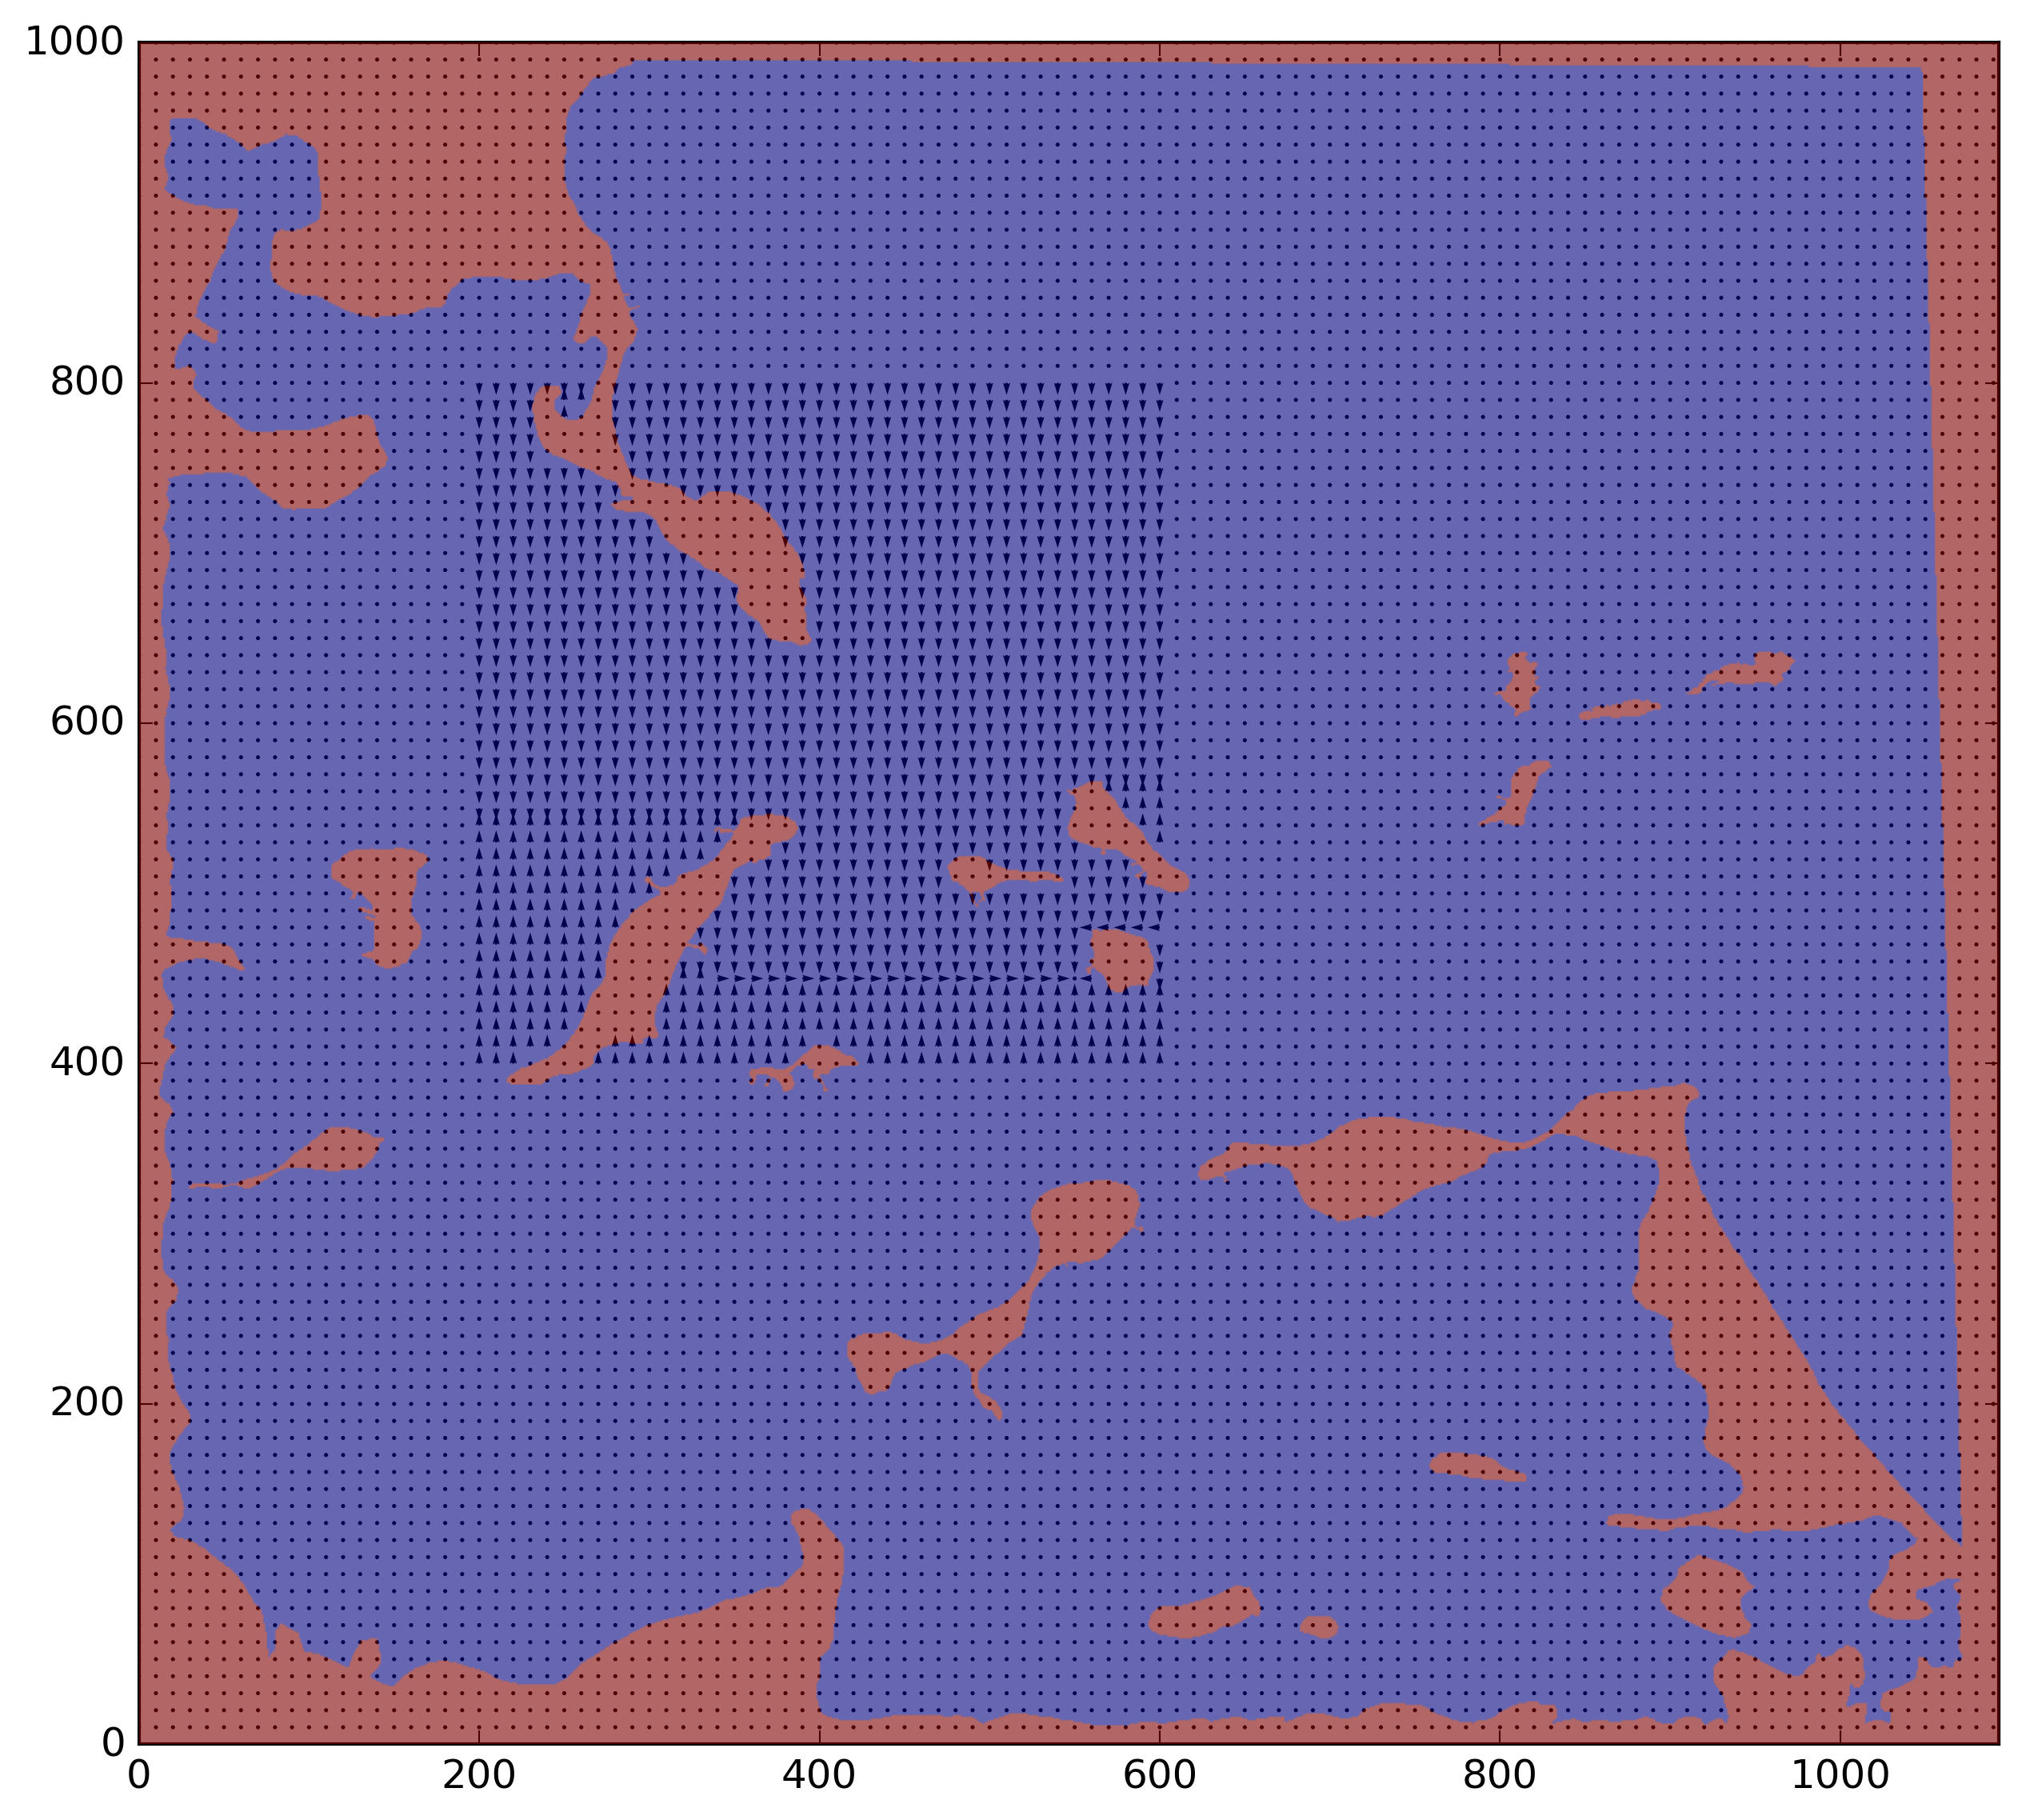
\includegraphics[width=\textwidth,trim={4cm 4cm 4cm 4cm},clip]{img/EXP7_history_plots_actions.png}
                \end{center}
            \end{block}
        \end{column}
        \begin{column}{0.33\textwidth}
            \begin{block}{Forces (certain)}
                \begin{center}
                      \includegraphics[width=\textwidth,trim={4cm 4cm 4cm 4cm},clip]{img/EXP6_history_plots_full_path.eps}
                \end{center}
            \end{block}
        \end{column}
        \begin{column}{0.33\textwidth}
            \begin{block}{Forces (uncertain)}
                \begin{center}
                      \includegraphics[width=\textwidth,trim={4cm 4cm 4cm 4cm},clip]{img/EXP5_history_plots_full_path.eps}
                \end{center}
            \end{block}
        \end{column}        
    \end{columns}
    \end{block}
\end{frame}


%%%%%
%%% Here
%%%%%


\begin{frame}{Results}
    \begin{columns}
        \begin{column}{0.5\textwidth}
            \begin{block}{Example Path}
                \begin{center}
                    % \includegraphics[width=\textwidth,trim={0cm 0cm 0cm 0cm},clip]{img/EXP5_history_plots_path.eps}
                \end{center}
            \end{block}
        \end{column}
        \begin{column}{0.5\textwidth}
            \begin{block}{Environment}
                \begin{center}
                    % \includegraphics[width=\textwidth,trim={0cm 0cm 0cm 0cm},clip]{img/EXP5_history_plots_full_path.eps}
                \end{center}
            \end{block}
        \end{column}
    \end{columns}
\end{frame}
\begin{frame}{Results}
    \begin{columns}
        \begin{column}{0.5\textwidth}
            \begin{block}{Applied Work}
                \begin{center}
                    \textbf{Image: applied work vector field}
                   %%% % \includegraphics[width=\textwidth,trim={0cm 0cm 0cm 0cm},clip]{img/applied_work}
                \end{center}
            \end{block}
        \end{column}
        \begin{column}{0.5\textwidth}
            \begin{block}{Actions as Vector Field}
                \begin{center}
                    \textbf{Image: Action grid}
                   %%% %\includegraphics[width=\textwidth,trim={0cm 0cm 0cm 0cm},clip]{img/actiongrid}
                \end{center}
            \end{block}
        \end{column}
    \end{columns}
\end{frame}
\begin{frame}{Results}
    \begin{columns}
        \begin{column}{0.5\textwidth}
            \begin{block}{Average cost2go}
                \begin{center}
                    % 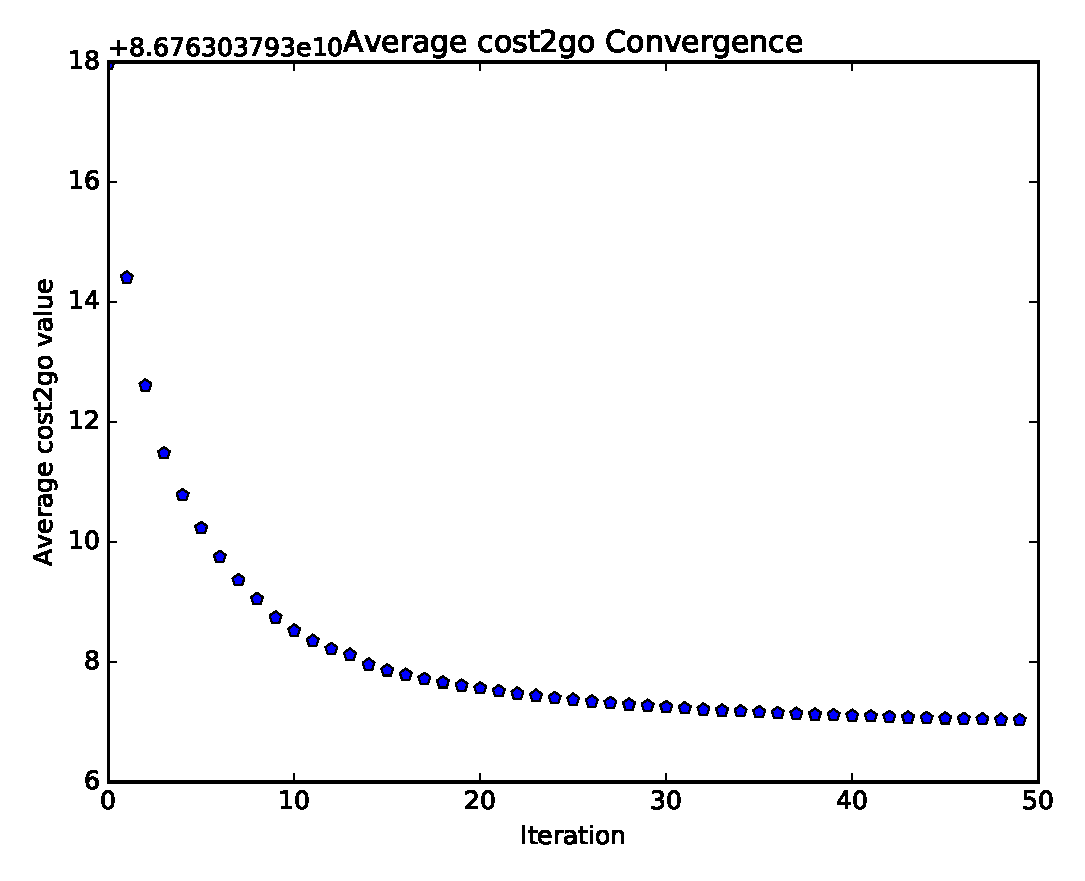
\includegraphics[width=\textwidth,trim={0cm 0cm 0cm 0cm},clip]{img/EXP5_history_plots_avg.eps}
                \end{center}
            \end{block}
        \end{column}
        \begin{column}{0.5\textwidth}
            \begin{block}{Average Change in cost2go}
                \begin{center}
                    % 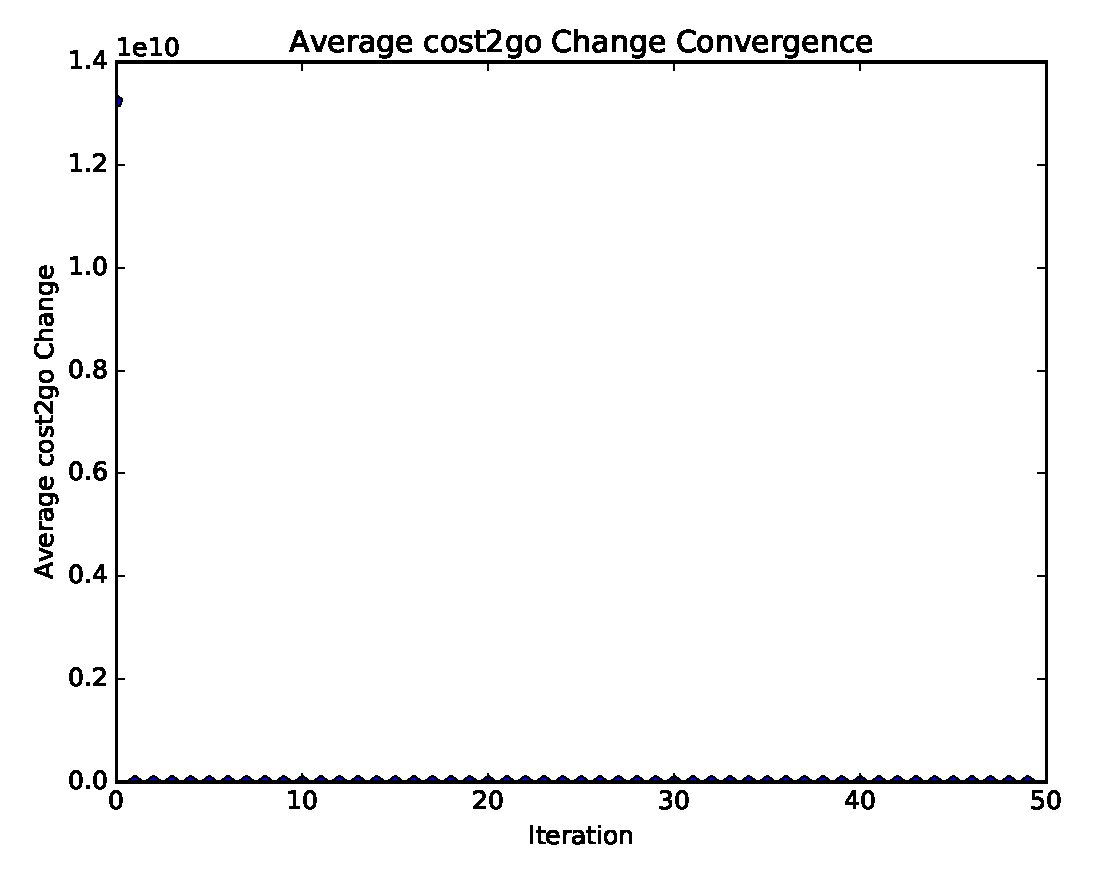
\includegraphics[width=\textwidth,trim={0cm 0cm 0cm 0cm},clip]{img/EXP5_history_plots_avg_diff.eps}
                \end{center}
            \end{block}
        \end{column}
    \end{columns}
\end{frame}
\begin{frame}{Results}
    \begin{columns}
        \begin{column}{0.33\textwidth}
            \begin{block}{Work}
                \begin{center}
                    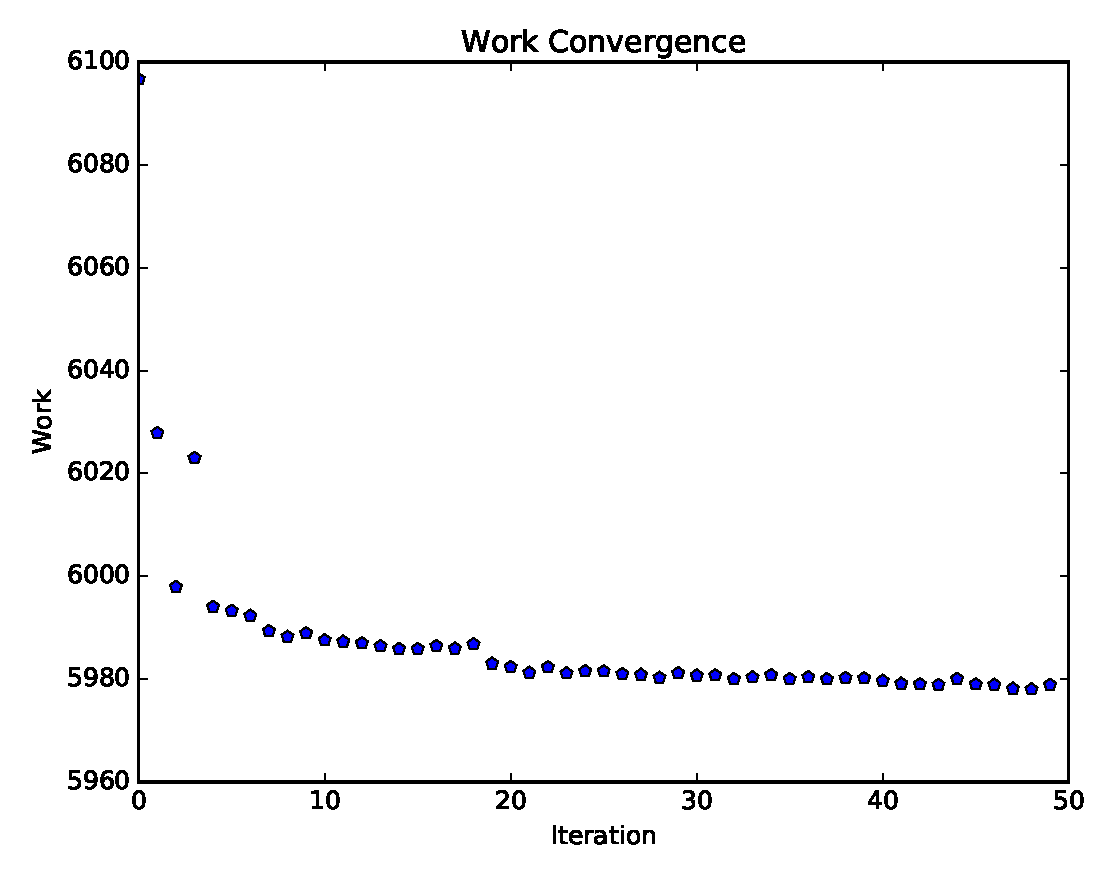
\includegraphics[width=\textwidth,trim={0cm 0cm 0cm 0cm},clip]{img/EXP5_history_plots_work.eps}
                \end{center}
            \end{block}
        \end{column}
        \begin{column}{0.33\textwidth}
            \begin{block}{Distance}
                \begin{center}
                    % 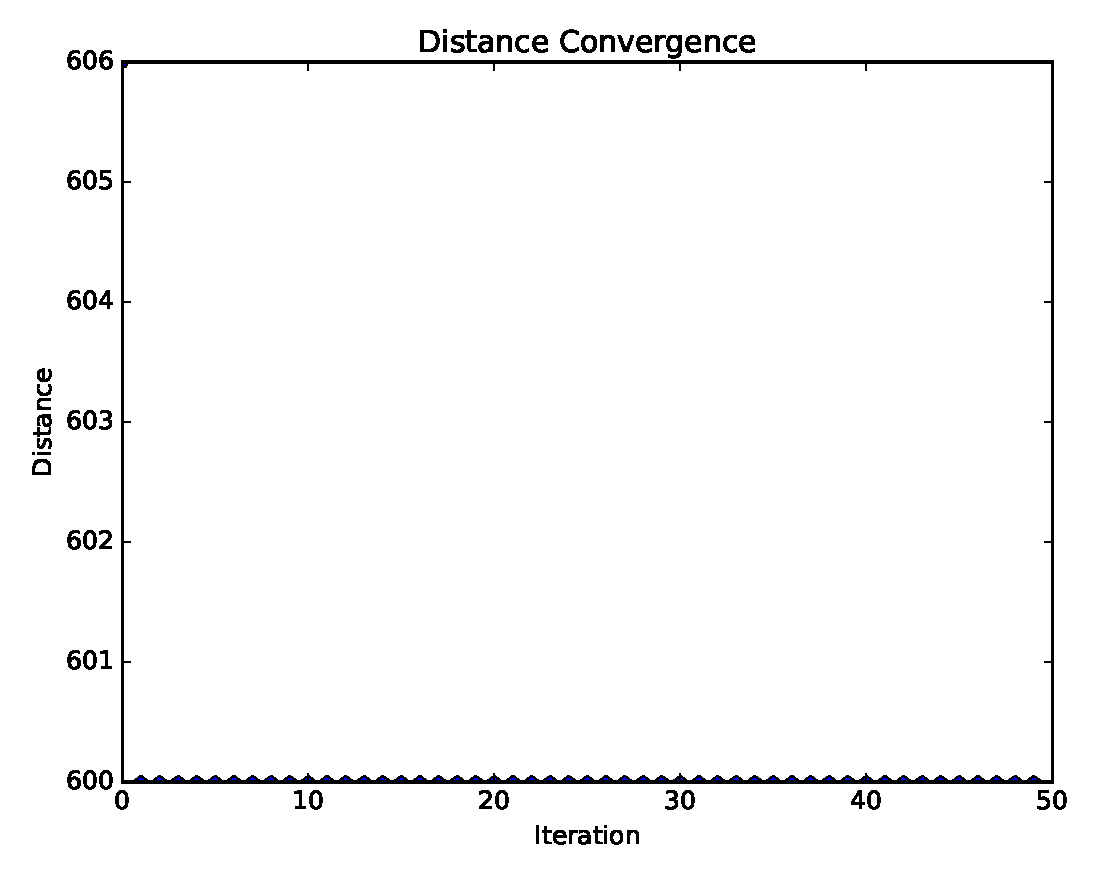
\includegraphics[width=\textwidth,trim={0cm 0cm 0cm 0cm},clip]{img/EXP5_history_plots_distance.eps}
                \end{center}
            \end{block}
        \end{column}
        \begin{column}{0.33\textwidth}
            \begin{block}{Number of Waypoints}
                \begin{center}
                    % 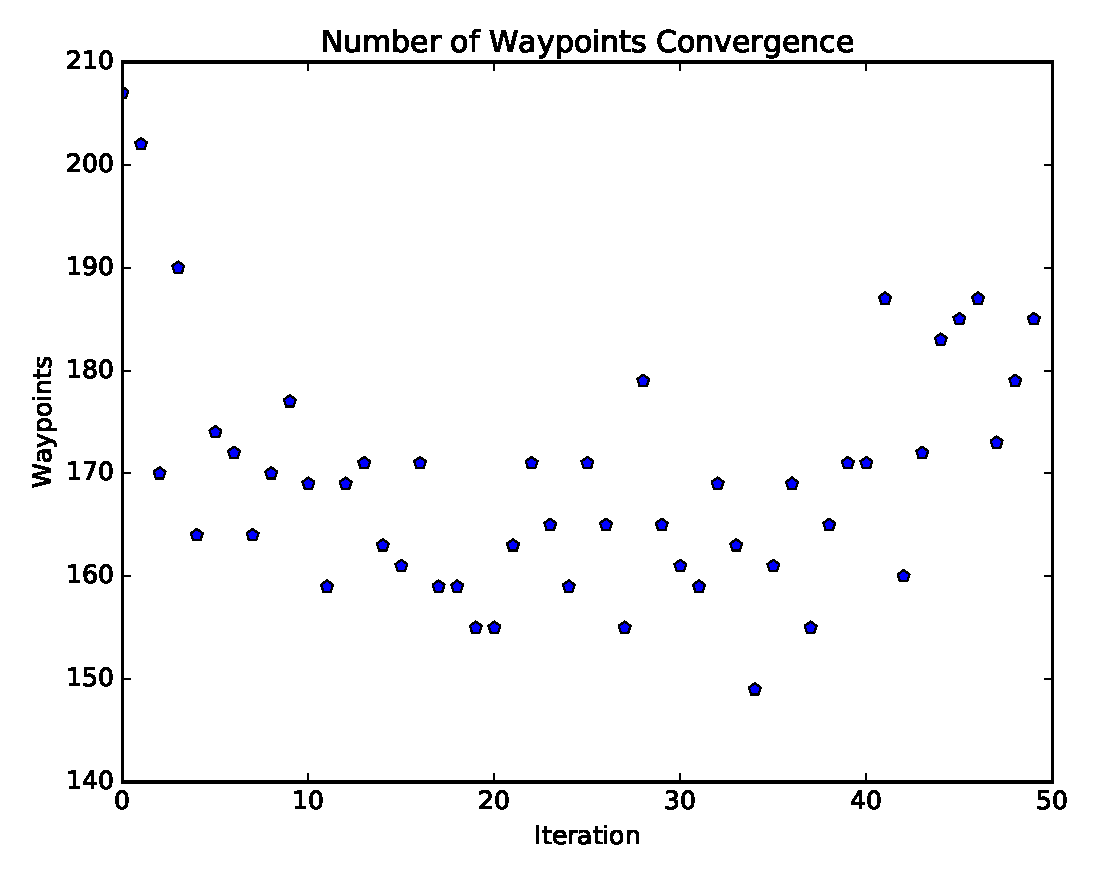
\includegraphics[width=\textwidth,trim={0cm 0cm 0cm 0cm},clip]{img/EXP5_history_plots_waypoints.eps}
                \end{center}
            \end{block}
        \end{column}
    \end{columns}
\end{frame}
\end{section}

\begin{section}{Conclusion \& Future Work}
\begin{frame}{Conclusions}
    \begin{itemize}
        \item Gives good paths
        \item Compared to traditional path planning..
    \end{itemize}
\end{frame}
\begin{frame}{Future Work}
    \begin{itemize}
        \item Compare to my metaheuristic planning results
        \item Implement with Gazebo
    \end{itemize}    
\end{frame}
\end{section}


\end{document}